\chapter{PINN-BO: A Black-Box Optimization
Algorithm Using Physics-Informed
Neural Networks} % Main chapter title
\label{chap:pinn-bo}
\section{Introduction}

In many scientific and engineering problems, the behavior of systems is often described by mathematical equations called \acfp{pde}. These equations represent fundamental physical laws, such as how heat spreads over time (the heat equation) or how fluids flow while considering factors like viscosity and external forces (the Navier-Stokes equations). \acp{pde} are essential tools in various fields, including structural analysis and electromagnetic, showing their broad importance.

Recently, researchers have tried to use \acp{pde} to improve the accuracy of modelling unknown functions. A common method uses \acp{gp} to combine information from observations of the objective function with the knowledge provided by \acp{pde}. While \acp{gp} are effective, they become slow and impractical for large datasets because their computations involve inverting large matrices, which can be very time-consuming.

To solve these challenges, \acfp{pinn} have been introduced. \acp{pinn} use neural networks to capture complex and nonlinear relationships, making them more flexible and scalable than \acp{gp}. \acp{pinn} can handle a wide variety of \acp{pde}, including nonlinear ones, and are better suited for large-scale problems in science and engineering.

While \acp{pde} offer useful information that can make optimization more efficient by reducing the need for expensive evaluations of the objective function. However, there is still limited research on how to effectively use \acp{pde} in \ac{bo}, where the objective function is unknown, noisy, or difficult to evaluate.

This chapter presents PINN-BO, a black-box optimization framework that employs a \ac{pinn} to model the unknown function, incorporates physical knowledge expressed by \acp{pde} constraints into the optimization process. Hence, PINN-BO aims to enhance model accuracy and improve constraint handling, particularly in problems governed by established physical laws. We summarize \textbf{the contributions of this chapter} as follows:
\begin{itemize}
    \item We introduce a novel black-box optimization problem with physics information, described by \acfp{pde}, which is used to govern the objective function.
    
    \item We propose PINN-BO, a black-box optimization algorithm employing \acl{pinn} with \acfp{pde} induced by natural laws to perform efficient optimization, bringing several benefits: improved sample-efficiency of optimization, scalable computation that only grows linearly with the number of function evaluations, and the ability to incorporate a broad class of \acp{pde}.
     
    \item We provide a theoretical analysis of our proposed PINN-BO algorithm to illustrate that incorporating linear \acp{pde} can lead to $\mathcal{O}\left(\sqrt{T\gamma_T}\sqrt{\gamma_T - I (f; \mathbf{Y}_T; \mathbf{U}_r) } \right)$ regret, where $T$ is the number of black-box function evaluations and $I (f; \mathbf{Y}_T; \mathbf{U}_r)$ is interaction information between the black-box function  $f$, its observations $\mathbf{Y}_T$ and the \ac{pde} data $\mathbf{U}_r$ (see Section \ref{section:pinn-bo_theoretical_analysis}).
    
    \item We perform experiments with a variety of tasks showing that our algorithm outperforms current state-of-the-art black-box optimization methods.
\end{itemize} 
This chapter begins by introducing the problem setting and give an example to illustrate our proposed setting, followed by a detailed description of the PINN-BO framework and its theoretical analysis.
 % For referencing the chapter elsewhere, use \ref{chap:background}
\section{Problem Setting}
\label{section:pinn-bo_problem_setting}
In this chapter, we consider a global optimization problem setting where the objective function $f \colon \mathcal{D} \rightarrow \mathbb{R}$ is associated with a \ac{pde}:   
\begin{equation*}
        \underset{\mathbf{x} \in \mathcal{D}}{\min} f(\mathbf{x}) \text{ s.t. }  \mathcal{N}[f](\mathbf{x}) = g(\mathbf{x}),
\end{equation*} 
where $\mathcal{D} \subset \mathbb{R}^d$ is a $d$-dimensional bounded domain and $\mathcal{N}[f]$ denotes a differential operator of the function $f$ with respect to the input $\mathbf{x}$. The function $f$ is an expensive, black-box function, and its evaluations are obtainable only through noisy measurements in the form of $y = f(\mathbf{x}) + \epsilon$, where $\epsilon$ represents sub-Gaussian noise. Additionally, the function $g(\mathbf{x})$ is a cheap-to-evaluate function, which may also involve noise, with respect to the \ac{pde}-constraint. Furthermore, it is assumed that the \textbf{boundary conditions} of the PDEs are either \textit{unknown or inaccessible}.
\begin{remark}
    Considering the damped harmonic oscillator from classical physics as a real-world example where $f(x)$ is the displacement of the oscillator as a black-box function of time $x$, and measuring the displacement of a damped harmonic oscillator accurately can be expensive due to several factors, e.g., instrumentation cost, environmental factors, and calibration requirements. This displacement is governed by the \ac{pde}: $m \frac{d^2f}{dx^2} + c \frac{df}{dx} + kf = 0$, where $\mathcal{N}[f](x) = m \frac{d^2f}{dx^2} + c \frac{df}{dx} + kf$, $g(x)=0$, $m, c, k$ are mass, damping and spring values, respectively. 
\end{remark}
\begin{remark}
    Assumptions about the \textit{unknown} or \textit{inaccessible} nature of boundary conditions are widely applicable across many problem settings. As an example, \citet{cai2020heat} examines a two-dimensional heat transfer problem with forced heat convection around a circular cylinder. The heat measurement entails high costs due to the material, size, and shape of the system. The problem has known incompressible Navier-Stokes and heat transfer equations. However, the thermal boundary conditions are difficult to ascertain precisely because of the complex and large instruments. The unavailability of these boundary conditions prevents the straightforward solution of the underlying function $f$ using traditional numerical techniques.
\end{remark}


\section{Proposed PINN-BO Method}
In this section, we present our proposed \ac{pinn} based \acl{bo} (PINN-BO). PINN-BO algorithm combines optimization and machine learning techniques to efficiently optimize an unknown black-box function over a given input space while leveraging physics-informed constraints described by a \ac{pde}. Following the fundamental principles of Bayesian optimization, our algorithm consists of two primary steps: (1) constructing a model of the black-box objective function, and (2) employing this model to select the next function evaluation point during each iteration. In the first step, our approach diverges from traditional Bayesian Optimization algorithms that typically utilize \acfp{gp} to model the objective function. Instead, we employ a fully connected neural network denoted as $h(\mathbf{x}; \boldsymbol{\theta})$ to learn the function $f$ as follows:
\[
h(\mathbf{x};\boldsymbol{\theta}) = \frac{1}{\sqrt{m}} \mathbf{W}_L \psi(\mathbf{W}_{L-1}\psi(\cdots \psi(\mathbf{W}_1 \mathbf{x})),
\]
where $\psi\colon \mathbb{R} \rightarrow \mathbb{R}$ is a coordinate-wise smooth activation function (e.g., ReLU, Tanh), $\mathbf{W}_1 \in \mathbb{R}^{m \times d}, \mathbf{W}_i \in \mathbb{R}^{m \times m}, 2\leq i \leq L-1, \mathbf{W}_L \in \mathbb{R}^{1 \times m}$, and $\boldsymbol{\theta} \in \mathbb{R}^p$ is the collection of parameters of the neural network, $p=md+m^2(L-2)+m$ and $d$ is the dimension of inputs, i.e., $\mathbf{x} \in \mathcal{D} \subset \mathbb{R}^d$. We initialize all the weights to be independent and identically distributed as standard normal distribution $\mathcal{N}(0,1)$ random variables. To leverage the information embedded within the \ac{pde} governing the objective function $f$, our algorithm generates a set of $N_r$ \ac{pde} data points denoted as $\mathcal{R} =  \{\mathbf{z}_j, u_j\}_{j=1}^{N_r}$. Here, $u_j$ represents the noisy evaluations of the function $g$ at the corresponding point $\mathbf{z}_j$, where $u_j = g(\mathbf{z}_j) + \eta_j$. Besides, we denote $\mathcal{D}_t = \{\mathbf{x}_i, y_i\}_{i=1}^t$ as the set of noisy observations of the unknown function $f$ after $t$ optimization iterations, where $y_t = f(\mathbf{x}_t) + \epsilon_t$. We further define some other notations:
\begin{equation*}
        \phi(\cdot) = \nabla_{\boldsymbol{\theta}} h(\cdot; \boldsymbol{\theta}_0) ; \; \; \; \;
        \omega(\cdot)  = \nabla_{\boldsymbol{\theta}} \mathcal{N}[h] (\cdot; \boldsymbol{\theta}_0)\\
\end{equation*}
where $\phi(\cdot)$ is the gradient of $h(\cdot; \boldsymbol{\theta}_0)$ with respect to the parameter $\boldsymbol{\theta}$, evaluated at initialization $\boldsymbol{\theta}_0$. Similarly, $\omega(\cdot)$ represents the gradient of $\mathcal{N}[h](\cdot; \boldsymbol{\theta}_0)$ with respect to model parameters $\boldsymbol{\theta}$ and evaluated at initialization $\boldsymbol{\theta}_0$, where $\mathcal{N}[h](\cdot; \boldsymbol{\theta}_0)$ is the result of applying differential operator $\mathcal{N}$ (with respect to the input) to $h(\cdot; \boldsymbol{\theta}_0)$. In our paper, we focus on cases where the differential operator \( \mathcal{N} \), when applied to a \textit{real-valued} function \( h \), produces another \textit{real-valued} function \( \mathcal{N}[h] \) (e.g., linear differential operator with real constant coefficients). 

Both $\mathcal{D}_t$ and $\mathcal{R}$ play an important role in the subsequent stages of the algorithm, specifically in the minimization of the loss function associated with learning the network $h(\mathbf{x}, \boldsymbol{\theta}_t)$ at optimization iteration $t$:
\begin{equation}
    \label{eqn:pinn_loss}
    \resizebox{0.9\textwidth}{!}{
$\mathcal{L}(t) = \sum^{t-1}_{i=1} [y_i - \nu_t h(\mathbf{x}_i; \boldsymbol{\theta}_{t-1})]^2 + \sum^{N_r}_{j=1}[u_j - \nu_t \mathcal{N}[h](\mathbf{z}_j; \boldsymbol{\theta}_{t-1})]^2$,
}
\end{equation}
where $\nu_t$ is a scale parameter that controls the exploration-exploitation trade-off. 

For the second step, we employ a greedy strategy to pick the next sample point $\mathbf{x}_t$. At each iteration $t$, the algorithm updates the neural network by optimizing the loss function described in Eqn \ref{eqn:pinn_loss} by gradient descent, with scaled function value predictions $\nu_t h(\cdot; \boldsymbol{\theta}_{t-1})$ and scaled predictions with respect to the governed \ac{pde} $\nu_t \mathcal{N}[h](\cdot; \boldsymbol{\theta}_{t-1})$. In the proof of Section \ref{section:pinn-bo_theoretical_analysis}, we show this action is equivalent to placing the \ac{gp} prior over function values $f_{1:t}$ and \ac{pde} values $g_{1:N_r}$ (Corollary \ref{corollary:pinn-bo_PINN_GP_func} in Appendix \ref{section:pinn-bo_supp}). 

The posterior distribution of the function prediction $\widetilde {f}_t(\mathbf{x}) = h(\mathbf{x}, \boldsymbol{\theta}_{t-1})$ at a new data point $\mathbf{x}$ can be viewed as being sampled from a \ac{gp} with specific posterior mean and variance function (Lemma \ref{lemma:pinn-bo_PINN_mean_cov}). This allows us to directly use the network prediction as an acquisition function following the principle of \acl{ts}.

The next evaluation point $\mathbf{x}_t$ is selected by minimizing this acquisition function $\widetilde {f}_t(\mathbf{x}) = h(\mathbf{x}, \boldsymbol{\theta}_{t-1})$. Then, the black-box function is queried at point $\mathbf{x}_t$, resulting in a (noisy) observation $y_t$, which is subsequently used to update the dataset $\mathcal{D}_t$. The \ac{pde} observations set $\mathcal{R}$, in combination with the observations in $\mathcal{D}_t$, is integrated into the training process of the neural network by minimizing the squared loss, as described in Eqn \ref{eqn:pinn_loss}. We provide a concise step-by-step summary of our approach in Algorithm \ref{alg:PINN-BO}.

To enhance the exploration step, it is important to bring the additional information to improve our model of objective function, especially in the regions where the optima are likely to be located. In our case, this task of exploration is easier as we have access to \ac{pde} which provides knowledge about the objective function and reduces the amount of information that is needed to model the function. In Section \ref{section:pinn-bo_theoretical_analysis} (Theoretical Analysis), we derive a scaling factor $\nu_t = B + \widetilde{R} \sqrt{2\gamma_t - 2 I(f; \mathbf{Y}_t; \mathbf{U}_r)  + \log(\frac{1}{\delta})}$,  which directly reflects this intuition. It reduces the maximum information gain  (which can be thought of as the complexity of the function modeling) by the interaction information $I(f; \mathbf{Y}_t; \mathbf{U}_r)$, which is a generalization of the mutual information for three variables: unknown function $f$,  its observations $\mathbf{Y}_t$, and the \ac{pde} data $\mathbf{U}_r$. This information can be calculated as $I(f; \mathbf{Y}_t; \mathbf{U}_r) = \frac{1}{2}  \log (\frac{\det(\frac{\boldsymbol{\Phi}_t^\top \boldsymbol{\Phi}_t}{\lambda_1} + \mathbf{I})\det(\frac{\boldsymbol{\Omega}_r^\top \boldsymbol{\Omega}_r}{\lambda_2} + \mathbf{I})}{\det(\frac{\boldsymbol{\Phi}_t^\top \boldsymbol{\Phi}_t}{\lambda_1} + \frac{\boldsymbol{\Omega}_r^\top \boldsymbol{\Omega}_r}{\lambda_2} + \mathbf{I})}) $, where $\boldsymbol{\Phi}_t  = [\phi(\mathbf{x}_1)^\top,\dots, \phi(\mathbf{x}_t)^\top ]$ and 
$\boldsymbol{\Omega}_r  = [\omega(\mathbf{z}_1)^\top, \dots, \omega(\mathbf{z}_{N_r})^\top ]$. The value of $\nu_t$ signifies how our algorithm continues the exploration in regions of search space where the function $f$ has no implicit knowledge through \ac{pde} observations. These are the regions indicated by $\gamma_t - I(f; \mathbf{Y}_t; \mathbf{U}_r)$, which is the amount of information about the unknown function $f$ remains after our algorithm interacts with \ac{pde} data $\mathbf{U}_r$.  

\begin{algorithm}[!ht]
\caption{Physics-informed Neural Network based Black-box optimization (PINN-BO)}
\label{alg:PINN-BO}
\textbf{Input}: The input space $\mathcal D$, the optimization budget $T$, \ac{pde} training set size $N_r$, $\delta \in (0,1)$, parameters $B, R_1, R_2, \lambda_1, \lambda_2$ (see Assumption \ref{assumption:pinn-bo_subgaussian} and \ref{assumption:pinn-bo_rkhs} in Section \ref{section:pinn-bo_theoretical_analysis}).
\begin{algorithmic}[1]
\State Initialize $\mathcal{D}_0 = \emptyset$ and $\boldsymbol{\theta}_0 \sim \mathcal{N}(\mathbf{0},\mathbf{I})$ 
\State Generate set $\mathcal{R} = \{\mathbf{z}_j, u_j\}_{j=1}^{N_r}$ from the \ac{pde}.

\For{$t = 1$ to $T$}
\State Set $\nu_t = B + \widetilde{R} \sqrt{2\gamma_t - 2 I(f; \mathbf{Y}_t; \mathbf{U}_r)  + \log(\frac{1}{\delta})}$, where $\widetilde{R} = \sqrt{\left(\frac{R_1}{\lambda_1}\right)^2 + \left(\frac{R_2}{\lambda_2}\right)^2}$. 
\State $\widetilde{f_t}(\mathbf{x}) = h(\mathbf{x}; \boldsymbol{\theta}_{t-1})$ 
\State Choose $\mathbf{x}_t = \argmin_{\mathbf{x} \in \mathcal{D}} \widetilde{f_t}(\mathbf{x}) $ and receive observation $y_t = f(\mathbf{x}_t) + \epsilon_t$
\State Update $\mathcal{D}_t = \mathcal{D}_{t-1} \cup \{\mathbf{x}_t, y_t\}$
\State Update $ \boldsymbol{\theta}_t = \argmin_{\boldsymbol{\theta}} \mathcal{L}(\boldsymbol{\theta})$ using Eqn. \ref{eqn:pinn_loss} by gradient descent with $\nu = \nu_t$.
\EndFor
\end{algorithmic}
\end{algorithm}


\section{Theoretical Analysis}
\label{section:pinn-bo_theoretical_analysis}

In this section, we provide a regret bound for the proposed PINN-BO algorithm. As presented in Section \ref{background:performance_metrics}, to quantify the algorithm's regret, we employ the cumulative regret, defined as $R_T = \sum_{t=1}^T r_t$ after $T$ iterations. Here, $\mathbf{x}^* = \argmin_{\mathbf{x} \in \mathcal{D}} f(\mathbf{x})$ represents the optimal point of the unknown function $f$, and $r_t = f(\mathbf{x^*}) - f(\mathbf{x}_t)$ denotes the instantaneous regret incurred at time $t$. Our regret analysis is built upon the recent NTK-based theoretical work of \citet{wang2022and} and proof techniques of GP-TS in \citet{chowdhury2017kernelized}. Before proceeding with the theoretical analysis, we now introduce a set of definitions and assumptions. They clarify our proof and set up the basis and conditions for our analysis. \textbf{A detailed proof can be found in Section \ref{section:pinn-bo_theoretical_analysis} of the Appendix.}   
\begin{definition}
    We define matrix $\mathbf{K}_\mathrm{NTK-PINN}$ as  the \textit{neural tangent kernel of a Physics-Informed Neural Network (NTK of PINNs)}: 
\begin{equation}
\renewcommand\arraystretch{1.2}
    \label{definition:PINN-NTKs}
\mathbf{K}_\mathrm{NTK-PINN} = 
\begin{bmatrix}
    \mathbf{K}_{uu} & \mathbf{K}_{ur} \\
    \mathbf{K}_{ru} & \mathbf{K}_{rr}
\end{bmatrix},
\end{equation}
where $(\mathbf{K}_{uu})_{ij} = \langle \phi(\mathbf{x}_i), \phi(\mathbf{x}_j) \rangle, 
 (\mathbf{K}_{ur})_{ij} = \langle \phi(\mathbf{x}_i), \omega(\mathbf{z}_j) \rangle, (\mathbf{K}_{rr})_{ij} = \langle \omega(\mathbf{z}_i), \omega(\mathbf{z}_j) \rangle$ and $\mathbf{K}_{ru} = \mathbf{K}_{ur}^\top$, defined using $\mathcal{D}_t$ and $\mathcal R$. 
\end{definition}

 \begin{assumption}
 \label{assumption:pinn-bo_subgaussian}
 We assume the noises $\{\epsilon_i\}_{i=1}^T$ where $\epsilon_i = y_i - f(\mathbf{x}_i)$ and $\{\eta_j\}_{j=1}^{N_r}$ where $\eta_j = u_j - g(\mathbf{z}_j)$  are conditionally sub-Gaussian with parameter $R_1 > 0$ and $R_2 >0$, where $\{\epsilon_i\}_{i=1}^T$ and $\{\eta_j\}_{j=1}^{N_r}$ is assumed to capture the noises induced by querying the black-box, expensive function $f(\cdot)$  and cheap-to-evaluate \ac{pde}-related function $g(\cdot)$ respectively. 
 \begin{equation*}
     \begin{split}
         \forall i \ge 0, & \; \forall \lambda_1 \in \mathbb{R}, \;  \mathbb{E}[e^{\lambda_1\epsilon_i} \rvert \mathcal{F}_{t-1}] \le e^\frac{\lambda_1^2 R_1^2}{2} \\
         \forall j \ge 0, & \; \forall \lambda_2 \in \mathbb{R}, \;  \mathbb{E}[e^{\lambda_2\eta_j} \rvert \mathcal{F}_{N_r-1}^\prime] \le e^\frac{\lambda_2^2 R_2^2}{2}
     \end{split}
 \end{equation*}
where $\mathcal{F}_{t-1}, \mathcal{F}_{N_r-1}^\prime$ are the $\sigma$-algebra generated by the random variables $\{\mathbf{x}_i, \epsilon_i\} 
^{t-1}_{i=1} \cup \{\mathbf{x}_t\}$ and $\{\mathbf{z}_j, \eta_j\} 
^{N_r-1}_{j=1} \cup \{\mathbf{z}_{N_r}\}$, respectively.
 \end{assumption}
 \begin{assumption}
    \label{assumption:pinn-bo_rkhs}
     We assume $f$ to be an element of the \acf{rkhs} associated with real-valued functions defined on the set $\mathcal{D}$ (For more details about \ac{rkhs}, see Section \ref{background:rkhs}). This specific \ac{rkhs} corresponds to the \acf{ntk} of a physics-informed neural network (NTK-PINN) and possesses a bounded norm denoted as $\norm{f}_{\mathcal{H}_{k_\textup{NTK-PINN}}} \leq B$.  Formally, this \ac{rkhs} is denoted as $\mathcal{H}_{k_\textup{NTK-PINN}}(\mathcal D)$, and is uniquely characterized by its kernel function $k_\textup{NTK-PINN}(\cdot, \cdot)$. The \ac{rkhs} induces an inner product $\langle \cdot, \cdot \rangle$ that obeys the reproducing property:
    $f(\mathbf{x}) = \langle f, k_\textup{NTK-PINN}(\cdot, \mathbf{x})\rangle$ for all $f \in  \mathcal{H}_{k_\textup{NTK-PINN}}(\mathcal{D})$. 
    The norm induced within this \ac{rkhs}, $\norm{f}_{\mathcal{H}_{k_\textup{NTK-PINN}}} = \sqrt{\langle f,f\rangle_{\mathcal{H}_{k_\textup{NTK-PINN}}}}$, quantifies the smoothness of $f$ concerning the kernel function $k_\textup{NTK-PINN}$, and satisfies: $f \in \mathcal{H}_{k_\textup{NTK-PINN}}(\mathcal{D})$ if and only if $\norm{f}_{k_{\mathcal{H}_\textup{NTK-PINN}}} < \infty$. 
 \end{assumption}


Assumptions \ref{assumption:pinn-bo_subgaussian} and \ref{assumption:pinn-bo_rkhs} represent commonly employed and well-established assumptions in GP-based Bandits and Bayesian Optimization \citep{chowdhury2017kernelized,vakili2021optimal}. We are now prepared to establish an upper bound on the regret incurred by our proposed PINN-BO algorithm.  

We begin by presenting key lemmas for establishing the regret bound in Theorem \ref{theorem:pinn-bo_regret_bound} of the proposed algorithms. The following lemma demonstrates that, given the assumption of an infinitely wide network, the output of the trained physics-informed neural network used to model the unknown function $f$ governed by a linear \ac{pde}, after running $t$ optimization iterations in Algorithm \ref{alg:PINN-BO}, can be regarded as sampling from a \ac{gp} with specific mean and covariance functions.
\begin{restatable}{lemma}{PinnMeanCov} 
\label{lemma:pinn-bo_PINN_mean_cov}
Conditioned on $\mathcal{D}_t = \{\mathbf{x}_i, y_i\}_{i=1}^t, \mathcal{R} = \{\mathbf{z}_j, u_j\}_{j=1}^{N_r}$, the acquisition function $\widetilde{f}_t(\mathbf{x}) = h(\mathbf{x}; \boldsymbol{\theta}_{t-1})$ can be viewed as a random draw from a $\mathrm{GP}\left(\mu_{t}^f (\mathbf{x}), \nu_t^2 \left(\sigma^f_t\right)^2(\mathbf{x})\right)$ with the following mean and covariance functions:
\begin{equation*}
\begin{split}
     \mu_{t}^f (\mathbf{x}) &= \phi(\mathbf{x})^\top \boldsymbol{\xi}_t^\top \mathbf{\widehat{K}}_\mathrm{PINN}^{-1} 
     \renewcommand\arraystretch{1.2}
     \begin{bmatrix}
         \mathbf{Y}_t \\
         \mathbf{U}_r
     \end{bmatrix} \\
    \left(\sigma^f_t\right)^2(\mathbf{x}) &=  \langle \phi(\mathbf{x}),  \phi(\mathbf{x}) \rangle - \phi(\mathbf{x})^\top \boldsymbol{\xi}_t^\top \mathbf{\widehat{K}}_\mathrm{PINN}^{-1} \boldsymbol{\xi}_t \phi(\mathbf{x}), \\
\end{split}
\end{equation*}
where 
\begin{equation*}
    \renewcommand\arraystretch{1.2}
    \begin{split}
\mathbf{\widehat{K}}_\mathrm{PINN}^{-1} &=  
    \begin{bmatrix}
    \mathbf{K}_{uu} + \lambda_1 \mathbf{I} & \mathbf{K}_{ur} \\
    \mathbf{K}_{ru} & \mathbf{K}_{rr} + \lambda_2 \mathbf{I}
    \end{bmatrix} ^{-1}  = \begin{bmatrix}
    \widetilde{\mathbf{A}} & \widetilde{\mathbf{B}} \\
    \widetilde{\mathbf{C}} & \widetilde{\mathbf{D}}
    \end{bmatrix}\\
    \boldsymbol{\Phi}_t & = [\phi(\mathbf{x}_1)^\top,\dots, \phi(\mathbf{x}_t)^\top ]  
\\
    \boldsymbol{\Omega}_r & = [\omega(\mathbf{z}_1)^\top, \dots, \omega(\mathbf{z}_{N_r})^\top ] \\ 
 \boldsymbol{\xi}_t &= \begin{bmatrix}
    \boldsymbol{\Phi}_t^\top & \boldsymbol{\Omega}_r^\top  
    \end{bmatrix}^\top 
\\
    \mathbf{K}_{uu} &= \boldsymbol{\Phi}_t \boldsymbol{\Phi}_t^\top, \;  \mathbf{K}_{ur} = \boldsymbol{\Phi}_t \boldsymbol{\Omega}_r^\top, \;
    \mathbf{K}_{ru} = \mathbf{K}_{ur}^\top, \mathbf{K}_{rr} = \boldsymbol{\Omega}_r \boldsymbol{\Omega}_r^\top 
\\
    \mathbf{Y}_t &= [y_1, y_2, \dots, y_t]^\top, 
    \mathbf{U}_r = [u_1, u_2, \dots, u_{N_r}]^\top \\
    \end{split}
\end{equation*}
\end{restatable}

Generic \ac{bo} methods (without the extra information from \ac{pde}) utilized the \textit{maximum information gain} over search space $\mathcal{D}$ at time $t$:
    $\gamma_t := \max_{\mathcal{A} \subset \mathcal{D}: \lvert \mathcal{A} \rvert=t} I(\mathbf{Y}_\mathcal{A}, f_\mathcal{A})$, 
    where $I(\mathbf{Y}_\mathcal{A}, f_\mathcal{A})$ denotes the mutual information between $f_\mathcal{A} = [f(\mathbf{x})]_{\mathbf{x}\in \mathcal{A}}$ and noisy observations $\mathbf{Y}_\mathcal{A}$, which quantifies the reduction in uncertainty about the objective function $f$ after observing $y_A$. The maximum information gain is the fundamental component when analyzing regret bound for their algorithm \citep{srinivas2009gaussian,vakili2021optimal}. Further details on this concept can be found in Section \ref{section:MIG}. However, in our work, the \ac{pde} evaluations $\{u_j\}_{j=1}^{N_r}$ of the function $g$ is considered as the second source of information that contributes to reduce the uncertainty of $f$. Therefore, we introduce the \textit{interaction information} as the generalization of \textit{mutual information} for three random variables:
\begin{definition}
\label{def:pinn-bo_interaction_information}
The \textbf{interaction information} between $f$,  its observations $\mathbf{Y}_\mathcal{A}$, (where $ \mathcal{A} \subset \mathcal{D}$), and the \ac{pde} data $\mathbf{U}_r$ can be defined as:
\[
I (f; \mathbf{Y}_\mathcal{A}; \mathbf{U}_r) = I (f; \mathbf{Y}_\mathcal{A}) - I (f; \mathbf{Y}_\mathcal{A} \rvert \mathbf{U}_r),
\]
where $I(f; \mathbf{Y}_\mathcal{A})$ quantifies the reduction in uncertainty in $f$ due to observing $\mathbf{Y}_\mathcal{A}$, while $I(f; \mathbf{Y}_\mathcal{A} \rvert \mathbf{U}_r)$ represents the additional information contributed by $\mathbf{U}_r$ to enhance the mutual information between $f$ and $\mathbf{Y}_\mathcal{A}$. 
\end{definition}
The next lemma provides the closed-form expression of the interaction information. 
\begin{restatable}{lemma}{InteractionInformation} 
    \label{lemma:pinn-bo_interaction_information_formula}
    The interaction information between $f$ and observation $\mathbf{Y}_t$ and \ac{pde} data $\mathbf{U}_r$, for the points chosen from Algorithm \ref{alg:PINN-BO} can be calculated as:
    \begin{equation*}
        I (f; \mathbf{Y}_t; \mathbf{U}_r) = \frac{1}{2}  \log (\frac{\det(\frac{\boldsymbol{\Phi}_t^\top \boldsymbol{\Phi}_t}{\lambda_1} + \mathbf{I})\det(\frac{\boldsymbol{\Omega}_r^\top \boldsymbol{\Omega}_r}{\lambda_2} + \mathbf{I})}{\det(\frac{\boldsymbol{\Phi}_t^\top \boldsymbol{\Phi}_t}{\lambda_1} + \frac{\boldsymbol{\Omega}_r^\top \boldsymbol{\Omega}_r}{\lambda_2} + \mathbf{I})})
    \end{equation*}
\end{restatable}

\begin{remark}
    \label{remark:pinn-bo_non_negative_interaction_information}
    Following Remark 3.3 in \citet{wang2022and}, both matrices $\frac{\boldsymbol{\Phi}_t^\top \boldsymbol{\Phi}_t}{\lambda_1}$ and $\frac{\boldsymbol{\Omega}_r^\top \boldsymbol{\Omega}_r}{\lambda_2}$ are positive semi-definite. It can be clearly seen that the interaction information given in Lemma \ref{lemma:pinn-bo_interaction_information_formula} is non-negative:
    \begin{equation*}
    \begin{aligned}
            I (f; \mathbf{Y}_t; \mathbf{U}_r) &= \frac{1}{2}  \log (\frac{\det(\frac{\boldsymbol{\Phi}_t^\top \boldsymbol{\Phi}_t}{\lambda_1} + \mathbf{I})\det(\frac{\boldsymbol{\Omega}_r^\top \boldsymbol{\Omega}_r}{\lambda_2} + \mathbf{I})}{\det(\frac{\boldsymbol{\Phi}_t^\top \boldsymbol{\Phi}_t}{\lambda_1} + \frac{\boldsymbol{\Omega}_r^\top \boldsymbol{\Omega}_r}{\lambda_2} + \mathbf{I})}) \\
            &= \frac{1}{2}  \log (\frac{\det(\frac{\boldsymbol{\Phi}_t^\top \boldsymbol{\Phi}_t}{\lambda_1} + \frac{\boldsymbol{\Omega}_r^\top \boldsymbol{\Omega}_r}{\lambda_2}  + \mathbf{I} + \frac{\boldsymbol{\Phi}_t^\top \boldsymbol{\Phi}_t \boldsymbol{\Omega}_r^\top \boldsymbol{\Omega}_r}{\lambda_1 \lambda_2})}{\det(\frac{\boldsymbol{\Phi}_t^\top \boldsymbol{\Phi}_t}{\lambda_1} + \frac{\boldsymbol{\Omega}_r^\top \boldsymbol{\Omega}_r}{\lambda_2} + \mathbf{I})}) \ge 0
        \end{aligned}
    \end{equation*}
    The inequality uses the identity $\det(\mathbf{A}+ \mathbf{B}) \ge \det(\mathbf{A})$, where $\mathbf{A},\mathbf{B}$ are two positive semi-definite matrices. 
\end{remark}
Our next result shows how the prediction of the neural network model is concentrated at the unknown reward function $f$ actual value, which is the key to a tighter regret bound.

\begin{restatable}{lemma}{PINNBOConfidenceBound}
\label{lemma:pinn-bo_confidence_bound}
     Assume that $\norm{\omega(\cdot)}_2 \le L$, where $\omega(\cdot)  = \nabla_{\boldsymbol{\theta}} \mathcal{N}[h] (\cdot; \boldsymbol{\theta}_0)$ and $\rho_{min}(\mathbf{K}_{uu})$ the smallest eigenvalue of kernel matrix $\mathbf{K}_{uu}$ defined in lemma 1. Set $N_r = c_r\left(1+ \frac{\rho_{min}(\mathbf{K}_{uu})}{\lambda_1}\right)/L^2$ for a positive constant $c_r$. Under the same hypotheses as stated in Assumption \ref{assumption:pinn-bo_subgaussian} and Assumption \ref{assumption:pinn-bo_rkhs}, and denote $\widetilde{R} = \sqrt{\left(\frac{R_1}{\lambda_1}\right)^2 + \left(\frac{R_2}{\lambda_2}\right)^2}$. Let $\delta \in (0,1)$. Then,  with  probability at least $1 - \delta$, the following confidence bound holds for all $\mathbf{x} \in \mathcal{D}$ and $t \ge 1$:
    \begin{equation*}
    \begin{aligned}
            & \lvert f(\mathbf{x}) - \mu_t^f(\mathbf{x}) \rvert \\
            & \le \sigma_t^f(\mathbf{x}) \left(B +   \widetilde{R}\sqrt{2 I (f; \mathbf{Y}_t) - 2I (f; \mathbf{Y}_t; \mathbf{U}_r) + \mathcal{O}(1) + \log(1/\delta)}  \right) \\
            & \le \sigma_t^f(\mathbf{x}) \left(B +   \widetilde{R}\sqrt{2 \gamma_t - 2I (f; \mathbf{Y}_t; \mathbf{U}_r) + \mathcal{O}(1) + \log(1/\delta)}  \right)
        \end{aligned}
    \end{equation*}
\end{restatable}
\paragraph{Proof sketch for Lemma \ref{lemma:pinn-bo_confidence_bound}}
We split the problem into two terms: The prediction error of an element $f$ in the \ac{rkhs} as assumed in Assumption \ref{assumption:pinn-bo_rkhs} with noise-free observations and the noise effect. Our proof differs from most GP-based Bayesian Optimization methods, which use single-block kernel matrices. In contrast, our predictive mean and covariance function involve the inversion of a block matrix  $\mathbf{\widehat{K}}_\mathrm{PINN}^{-1}$, as stated in Lemma \ref{lemma:pinn-bo_PINN_mean_cov}. We employ the block matrix inversion formula (see Appendix A, \citep{rasmussen2006gaussian}) to express $\mathbf{\widehat{K}}_\mathrm{PINN}^{-1}$ as four distinct matrices. Subsequently, using equivalent transformations, intermediate matrix identities, and utilizing the expression \textit{Interaction information} provided in Lemma \ref{lemma:pinn-bo_interaction_information_formula}, we derive the final bound. 

\begin{remark}
    The upper bound of the confidence interval presented in Lemma \ref{lemma:pinn-bo_confidence_bound} shares a similar form with the existing confidence interval of GP-TS as outlined in \citet{chowdhury2017kernelized}. It is worth emphasizing, however, that our bound offers valuable insights into the significance of integrating \acp{pde} to attain a tighter confidence bound. This insight can be summarized as follows: The expression $I(f; \mathbf{Y}_t) - I(f; \mathbf{Y}_t; \mathbf{U}_r)$ equals to $I(f; \mathbf{Y}_t|\mathbf{U}_r)$, which represents the expected mutual information between the function $f$ and the observations $\mathbf{Y}_t$, given $\mathbf{U}_r$. Lemma \ref{lemma:pinn-bo_interaction_information_formula} quantifies $I(f; \mathbf{Y}_t; \mathbf{U}_r)$ in terms of the kernel Gram matrices induced by black-box function and the \ac{pde} observations. As mentioned in Remark \ref{remark:pinn-bo_non_negative_interaction_information}, the condition $I(f; \mathbf{Y}_t; \mathbf{U}_r) \ge 0$ implies that $I(f; \mathbf{Y}_t) \ge I(f; \mathbf{Y}_t|\mathbf{U}_r)$.  This inequality signifies that knowing the values of the \ac{pde} component $\mathbf{U}_r$ reduces the statistical information between the observations $\mathbf{Y}_t$ and the unknown function $f$. In other words, knowing the values of \ac{pde} component $\mathbf{U}_r$ can diminish the number of observations $\mathbf{Y}_t$ required to estimate the unknown function $f$. 
\end{remark} 

\begin{remark}
The value of $I(f; \mathbf{Y}_t; \mathbf{U}r)$ depends on the specific problem. For instance, if we assume that $f$ is a function in \ac{rkhs} with a linear kernel and $\mathcal{N}[f]= \sum_{i=1}^n \frac{\partial f}{\partial \mathbf{x}_i}$, the lower bound for the interaction information is: \[
I(f; \mathbf{Y}_t; \mathbf{U}_r) = \Theta\left(\frac{d N_r}{d N_r+1}(1-1/T)\right) = \Theta(1),
\] 
which is a constant. This is because the linear kernel differential feature map sends all \ac{pde} points to the same vector in the \ac{rkhs}. This example aims to show how to bound the interaction information for a known \ac{pde}. 
\end{remark}
We are now ready to present the main theoretical result of the paper: 
\begin{restatable}{theorem}{PINNBORegretBound}
\label{theorem:pinn-bo_regret_bound}
Let $\mathbf{K}_{uu}, \mathbf{K}_{ur}, \mathbf{K}_{ru},$ and $\mathbf{K}_{rr}$ be four matrices as defined in Lemma \ref{lemma:pinn-bo_PINN_mean_cov}. 
Let $\delta \in (0,1)$. Assume that $\norm{\omega(\cdot)}_2 \le L$ and  $\rho_{min}(\mathbf{K}_{uu})$ be the smallest eigenvalue of kernel matrix $\mathbf{K}_{uu}$. Set $N_r = c_r\left(1+ \frac{\rho_{min}(\mathbf{K}_{uu})}{\lambda_1}\right)/L^2$ for a constant $c_r > 0$. Additionally,  let $\widetilde{R} = \sqrt{\left(\frac{R_1}{\lambda_1}\right)^2 + \left(\frac{R_2}{\lambda_2}\right)^2}$ and $I_0 = \frac{1}{2}\log \frac{\det(\mathbf{K}_{rr} + \lambda_2\mathbf{I})}{\det(\mathbf{K}_{rr} + \lambda_2\mathbf{I} - \mathbf{K}_{ru} \mathbf{K}_{uu}^{-1} \mathbf{K}_{ur})}$. Then with probability at least $1-\delta$, the regret of PINN-BO running for an unknown function $f$ governed by a linear \ac{pde}, lying in the $\mathcal{H}_{k_\textup{NTK-PINN}}$, $\norm{f}_{{H}_{k_\textup{NTK-PINN}}} \le B$ as stated in Assumption \ref{assumption:pinn-bo_rkhs}, after $T$ iterations satisfies:
\begin{equation*}
    \begin{aligned}
        R_T  = \mathcal{O} \Bigg(\sqrt{T d\log BdT} &\bigg[B \sqrt{\gamma_T - I_0 + \log(2/\delta)} 
        \\
        & + \widetilde{R} \sqrt{\gamma_T} \sqrt{\gamma_T - I (f; \mathbf{Y}_T; \mathbf{U}_r) - I_0 + \log(2/\delta
        )} \bigg] \Bigg)
    \end{aligned}
\end{equation*}
\end{restatable}


\section{Experiments}

In this section, we demonstrate the effectiveness of our proposed PINN-BO algorithm through its application of synthetic benchmark optimization functions as well as real-world optimization problems. Our implementations of both problems are available at: \url{https://github.com/phantrdat/neural-cbo}.  

\subsection{Experimental Setup}
\label{section:baselines}
For all experiments, we compared our algorithm with common classes of surrogate models used in black-box optimization, including Gaussian Processes (GPs) and Deep Neural Networks (DNNs). For GPs, we employ the most popular strategy GP-EI \citep{mockus1978application} and GP-UCB \citep{srinivas2009gaussian} with the Mat\'ern Kernel. Our implementations for GP-based Bayesian Optimization baselines utilize public library GPyTorch  \url{https://gpytorch.ai/} and BOTorch \url{https://botorch.org/}. We also include two recent DNNs-based works for black-box optimization: Neural Greedy \citep{pariagreedy} and Neural-BO \citep{phan2023neuralbo} described below:
\begin{itemize}
    \item Neural Greedy in \citet{pariagreedy} fits a neural network to the current set of observations, where the function values are randomly perturbed before learning the neural network. The learned neural network is then used as the acquisition function to determine the next query point. Since the NeuralGreedy code is not publicly available, we use our own implementation following the setting described in     \citet{pariagreedy} (see Appendix F.2 therein).
    \item NeuralBO in \citet{phan2023neuralbo} utilizes the \acl{ts} strategy for selecting the next evaluation point. In this approach, the mean function is estimated using the output of a fully connected deep neural network. To implement this baseline, we adhere to the configuration outlined in Section 7 in \citet{phan2023neuralbo}.
\end{itemize}
For our proposed PINN-BO algorithm, we employ a fully connected deep neural network (DNN) as the surrogate model. The network's weights are initialized with independent samples drawn from a normal distribution $\mathcal{N} (0, 1)$. The model's hyperparameters, which include depth, width, and learning rate, are selected as follows: For each function, we perform a grid search for tuning, where each hyperparameter tuple is trained with 50 initial points. The width is explored within the set $\{100,200,500\}$, while the depth and the learning rate are searched across the values $\{2,3,4\}$ and $\{0.001, 0.005, 0.01, 0.02, 0.05, 0.1\}$, respectively.  Subsequently, we select the tuple of (depth, width, learning rate) associated with the lowest mean-square error during evaluation. To train the surrogate neural network models, we utilize the (stochastic) gradient descent optimizer along with an Exponential Learning Rate scheduler with a factor of $\gamma=0.95$. To accelerate the training process, we update the parameters $\boldsymbol{\theta}_t$ of surrogate models in Algorithm \ref{alg:PINN-BO} after every 10 optimization iterations with 100 epochs.  

\subsection{Synthetic Benchmark Functions}
 We conducted optimization experiments on five synthetic functions: DropWave (2), Styblinski-Tang (10), Rastrigin (20), Michalewics (30), and Cosine Mixture (50), where the numbers in parentheses indicate the input dimensions of each function. We selected them to ensure a diverse range of difficulty levels, as suggested by the difficulty rankings available at \url{https://infinity77.net/global_optimization/test_functions.html}. To enhance the optimization process, we incorporated the \acp{pde} associated with these objective functions. The detailed expressions of these functions and their corresponding \acp{pde} can be found in  Section \ref{section:pinn-bo_experiments_synthetic}  of the  Appendix \ref{section:pinn-bo_supp}. Additionally, the noise in function evaluations follows a normal distribution with zero mean, and the variance is set to 1\% of the function range. Results for Rastrigin, Michalewics, and Cosine Mixture functions are presented in Figure \ref{fig:pinn-bo_synthetic}.
All experiments reported here are averaged over 10 runs, each with random initialization. All methods begin with the same initial points. The results demonstrate that our PINN-BO is better than all other baseline methods, including GP-based BO algorithms (GP-EI, GP-UCB), and NN-based BO algorithms (NeuralBO, NeuralGreedy). 


\begin{figure}[H] %
  \centering
  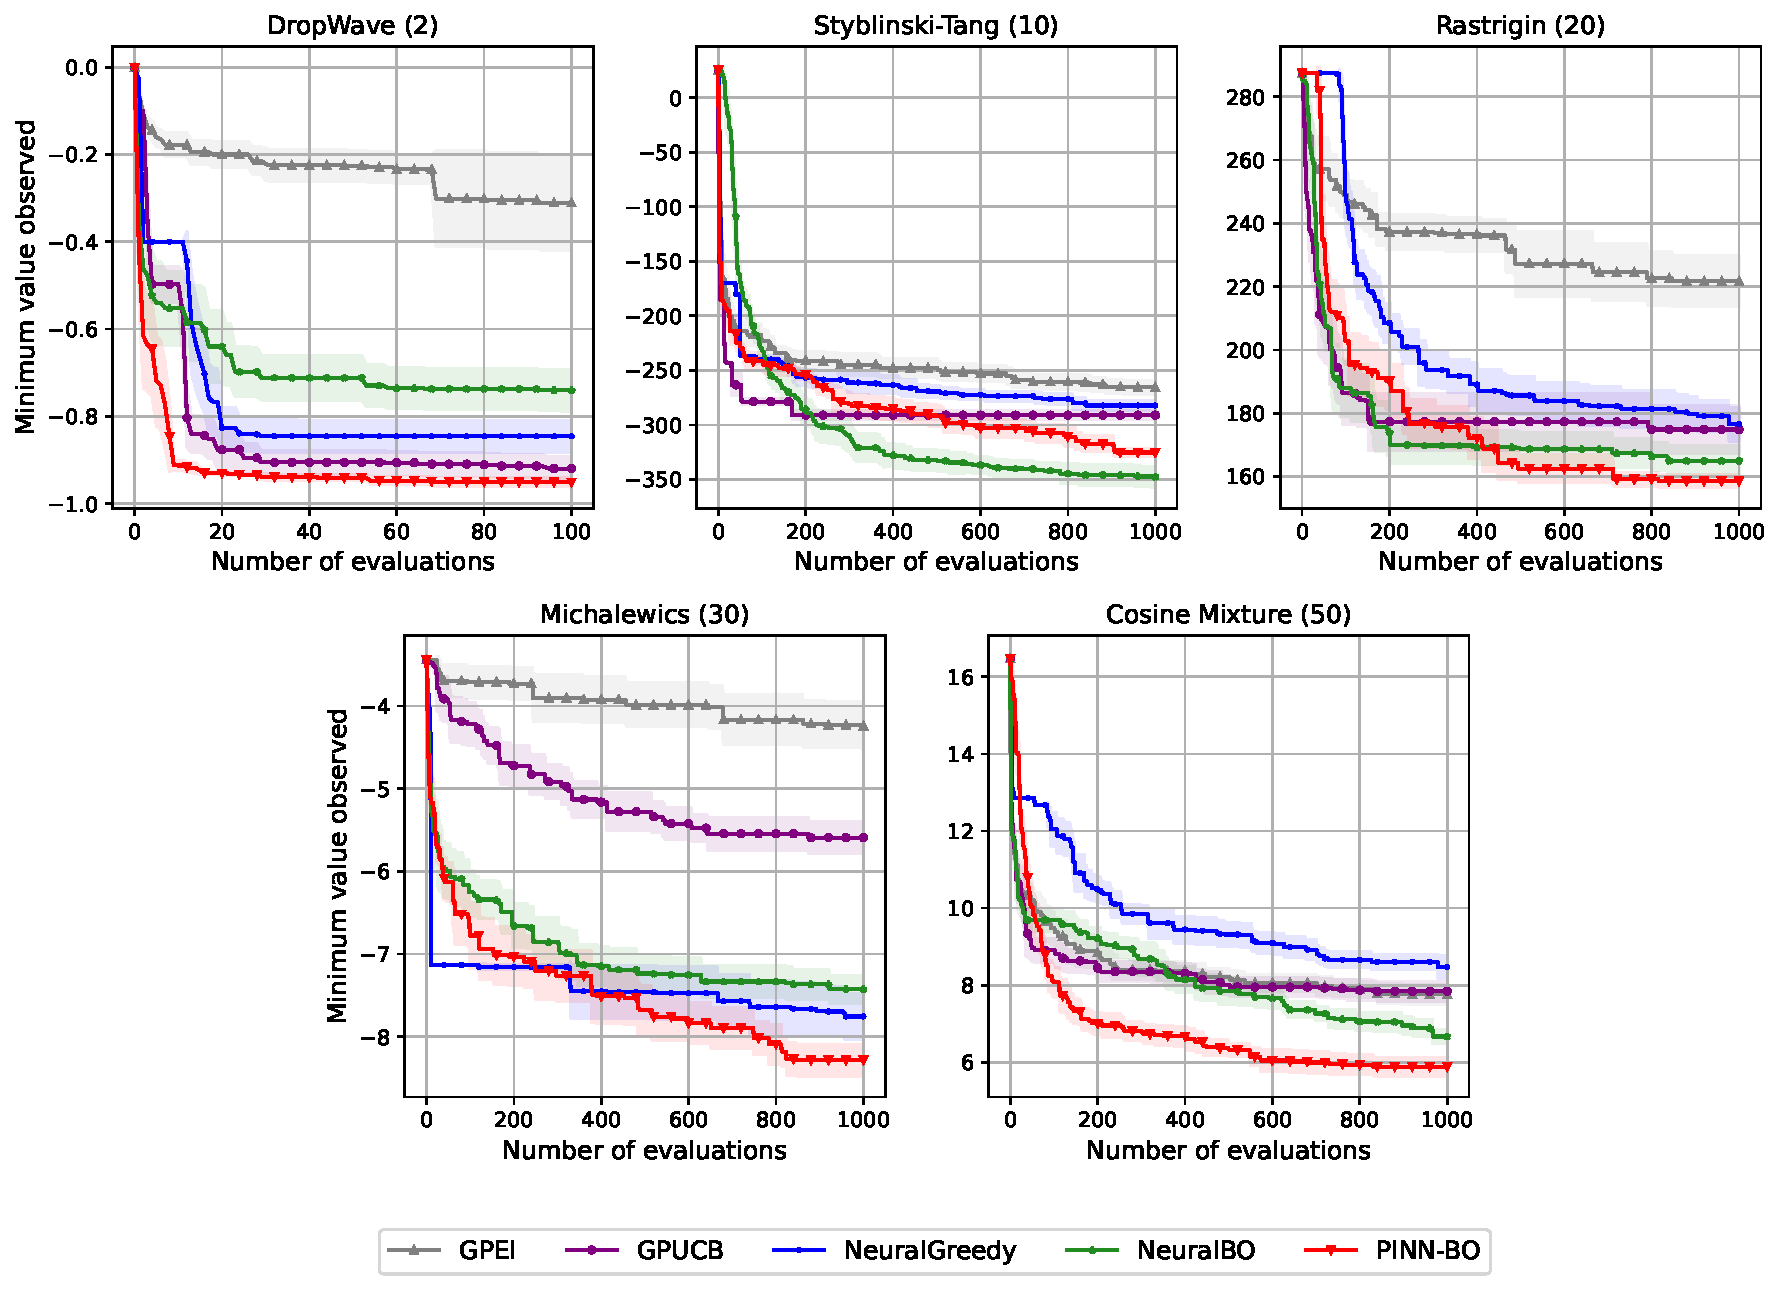
\includegraphics[width=\textwidth]{Figures/PINN-BO/pinn-bo_all_synthetic.pdf} 
  \caption{The optimization results for Rastrigin, Michalewics and Cosine Mixture, DropWave and Styblinski-Tang functions comparing the proposed PINN-BO with the baselines. The standard errors are shown by color shading.}
  \label{fig:pinn-bo_synthetic}
\end{figure}


\subsection{Real-world Applications}
In this section, we explore two real-world applications where the objective functions are constrained by specific \acp{pde}. We consider two tasks: (1) optimizing the Steady-State temperature distribution, satisfying the  Laplace equation, and (2) optimizing the displacement of a beam element, adhering to the non-uniform Euler-Bernoulli equation. We continue to compare our proposed method with the baselines mentioned in Section \ref{section:baselines}. 

\subsubsection{Optimizing Steady-State Temperature}
\label{section:pinn-bo_experiments_2d_laplace}
In this study, we showcase the benchmark optimization outcomes achieved by our proposed PINN-BO algorithm, comparing them with baseline methods for the steady-state temperature optimization task. The steady-state heat equation represents a special case of the heat equation when the temperature distribution no longer changes over time. It describes the equilibrium state of a system where the temperature is constant, and no heat is being added or removed.  The governing PDE for the temperature distribution is expressed as: $\nabla^2 T(x, y) = 0$, where $x, y$ are spatial variables that represent the positions within a two-dimensional space. We explore the heat equation in a domain where $x$ and $y$ lie within the defined range of $[0,2\pi]$. To thoroughly investigate the problem, we consider three different heat equations, where the solution of each problem is associated with one (unknown) boundary condition, each contributing to a deeper understanding of the system: 

 \paragraph{Heat Equation with Boundary Conditions 1}
 \label{para:heat1}
 \begin{align*}
     T(x, 0) &= 5\sin(y) + \sqrt{1+y} \\
    T(x, 2\pi) &= y\sin\left(3\cos(y) + 2\exp(y)\sin(y)\right) \\
   T(0, y) &= 10\cos(x) + x\exp(\sqrt{x^2 + \sin(x)}) \\
   T(2\pi, y) &= 3\sqrt{\exp(x\exp(-x))}\sin(x) + \cos(3x)\cos(3x)
 \end{align*}
 \paragraph{Heat Equation with Boundary Conditions 2}
 \label{para:heat2}
\begin{align*}
    T(x, 0) &= \sin(x) \cos(2x) + x^2\sqrt{3x}  + e^{\sin(x)} \\
    T(x, 2\pi) &= e^{\sin(x)} \sqrt{3x} + x^2 \cos(x)  \sin^2(x)   + e^{\cos(x)} \\
    T(0, y) &= \sqrt{2y}  \sin(y) + y^3\cos(2y)   + e^{\cos(y)} \\
    T(2\pi, y) &= \sin(y) \cos(2y) + y^3\sqrt{2y}   + e^{\sin(y)}
\end{align*}
\paragraph{Heat Equation with Boundary Conditions 3}
\label{para:heat3}
\begin{align*}
    T(x, 0) &= \left(\sin(x) + \cos(2x) \right) \sqrt{3x} + x^2 + e^{\sin(x)} \\
    T(x, 2\pi) &= \left(e^{\sin(x)} + \sqrt{3x} \right) \cos(x) + \left(\sin^2(x) + x^2\right)  e^{\cos(x)}
    \\
    T(0, y) &= \left(\sqrt{2y} + \sin(y)\right)  \left(\cos(2y) + y^3 \right) + e^{\cos(y)}\\
    T(2\pi, y) &= \left(\sin(y) + \cos(2y)\right) \left(\sqrt{2y} + y^3\right) + e^{\sin(y)}
\end{align*}
We utilized \texttt{py-pde}, a Python package designed for solving partial differential equations (PDEs), available at the following GitHub repository: \url{https://github.com/zwicker-group/py-pde}. This tool enabled us to obtain solutions to heat equations at various input points, with specific boundary conditions serving as the input data. In Figure \ref{fig:heat_dist}, the temperature distribution within the defined domain $[0, 2\pi]$ is visualized. It is important to emphasize that the boundary conditions used for benchmarking purposes are unknown to the methods employed. Adhering to the framework of black-box optimization, we assume that solving the PDEs incurs a substantial computational cost. The figure illustrates the spatial distribution of temperature values $T(x,y)$ across domain $[0, 2\pi] \times [0, 2\pi]$, with each subfigure corresponding to one of the mentioned boundary conditions.  
\begin{figure}[ht]
    \centering
    \begin{subfigure}[b]{0.49\textwidth}
        \centering
        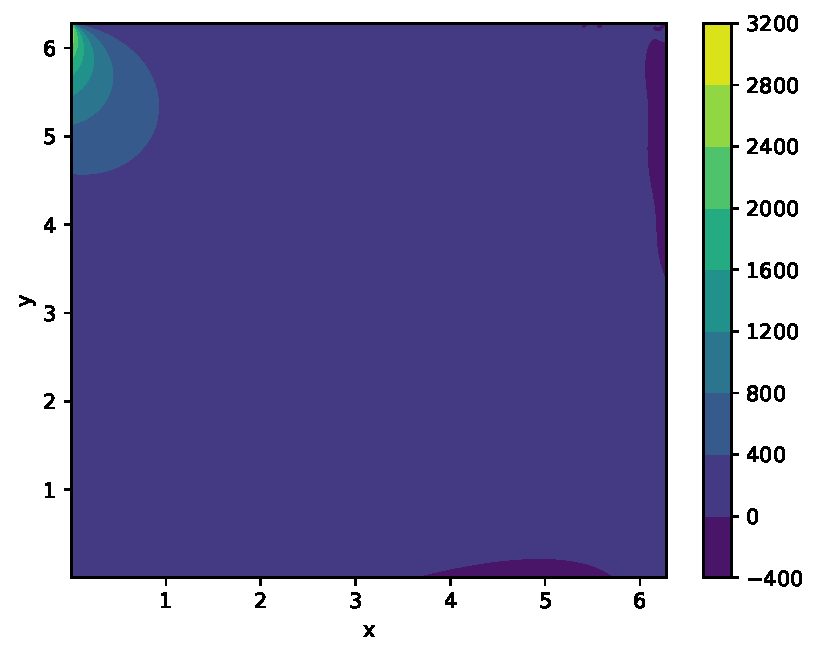
\includegraphics[width=\textwidth]{Figures/PINN-BO/heat_py_pde_1000_test_1.pdf}
        \caption{Solution of Temperature Equation with boundary conditions 1}
 \label{fig:heat_1_dist}
    \end{subfigure}
    \hfill
    \begin{subfigure}[b]{0.49\textwidth}
        \centering
        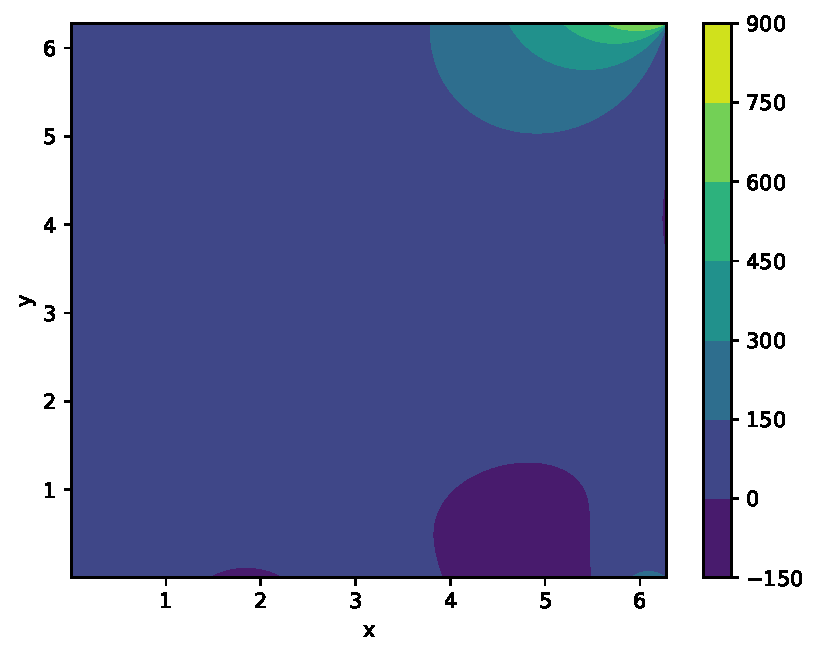
\includegraphics[width=1\textwidth]{Figures/PINN-BO/heat_py_pde_1000_test_2.pdf}
        \caption{Solution of Temperature Equation with boundary conditions 2}
        \label{fig:heat_2_dist}
    \end{subfigure}
    \hfill
    \begin{subfigure}[b]{0.5\textwidth}
        \centering
        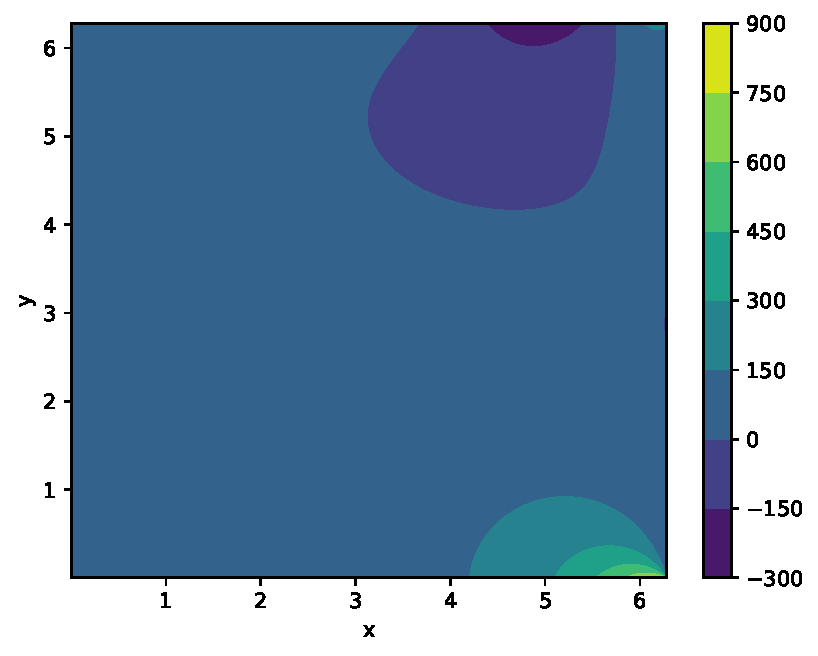
\includegraphics[width=\textwidth]{Figures/PINN-BO/heat_py_pde_1000_test_3.pdf}
        \caption{Solution of Temperature Equation with boundary conditions 3}
        \label{fig:heat_3_dist}
    \end{subfigure}
    \caption{The figures depict the solutions for temperature distributions governed by the heat equation, with each figure corresponding to a specific tuple of boundary conditions described in Section \ref{section:pinn-bo_experiments_2d_laplace}. It is evident that the region with the highest temperature is relatively small in comparison to the entire domain.}
    \label{fig:heat_dist}
\end{figure}

We conducted temperature optimization by identifying the locations $(x,y)$ where the temperature reaches its maximum. As illustrated in Figure \ref{fig:heat_dist}, the area with high temperatures is relatively small in comparison to the regions with medium or low temperatures. For each baseline, we performed the optimization process 10 times, computing the average results. The comparative outcomes are presented in Figure \ref{fig:heat_opt}. 
\begin{figure}[ht]
    \centering
    \begin{subfigure}[b]{0.49\textwidth}
        \centering
    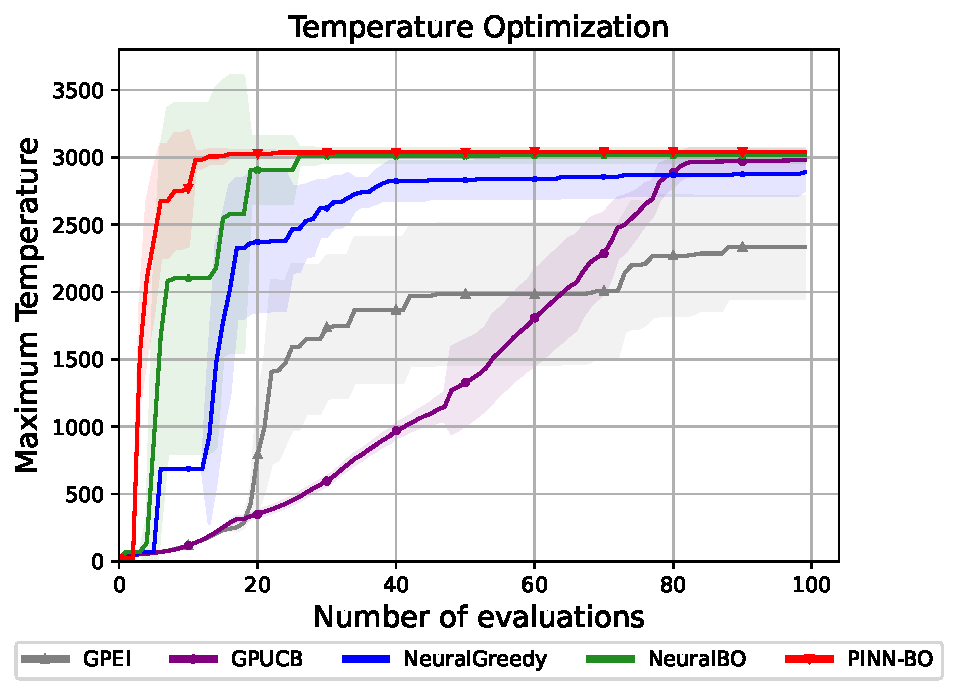
\includegraphics[width=\textwidth]{Figures/PINN-BO/Heat_dim_2_bc1.pdf}
        \caption{Temperature Optimization in case of boundary conditions 1}
 \label{fig:heat_1_opt}
    \end{subfigure}
    \hfill
    \begin{subfigure}[b]{0.49\textwidth}
        \centering
        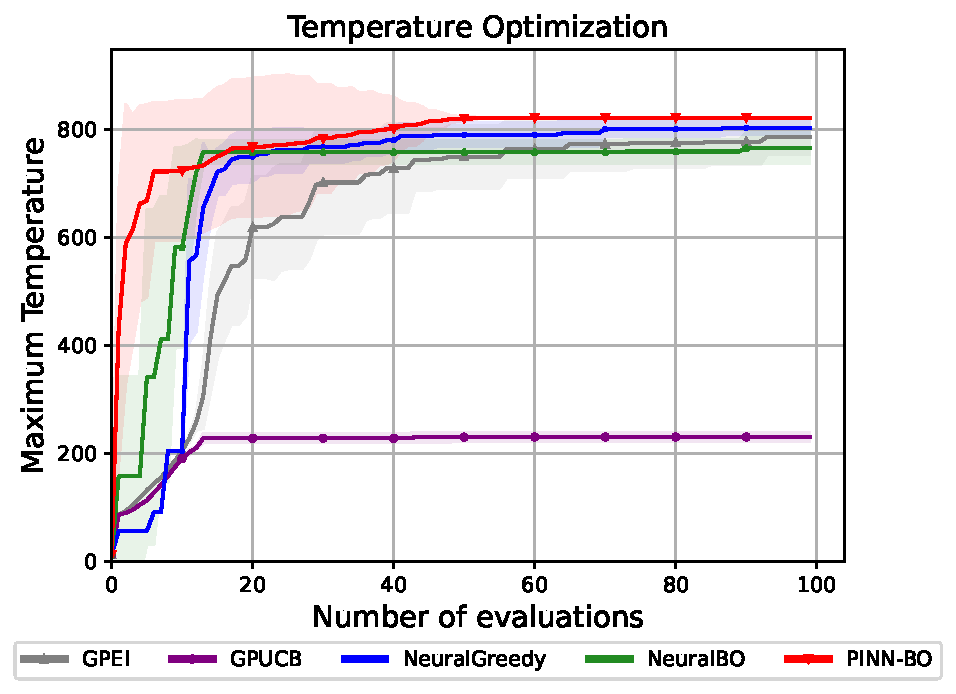
\includegraphics[width=1\textwidth]{Figures/PINN-BO/Heat_dim_2_bc2.pdf}
        \caption{Temperature Optimization in case of boundary conditions 2}
        \label{fig:heat_2_opt}
    \end{subfigure}
    \hfill
    \begin{subfigure}[b]{0.5\textwidth}
        \centering
        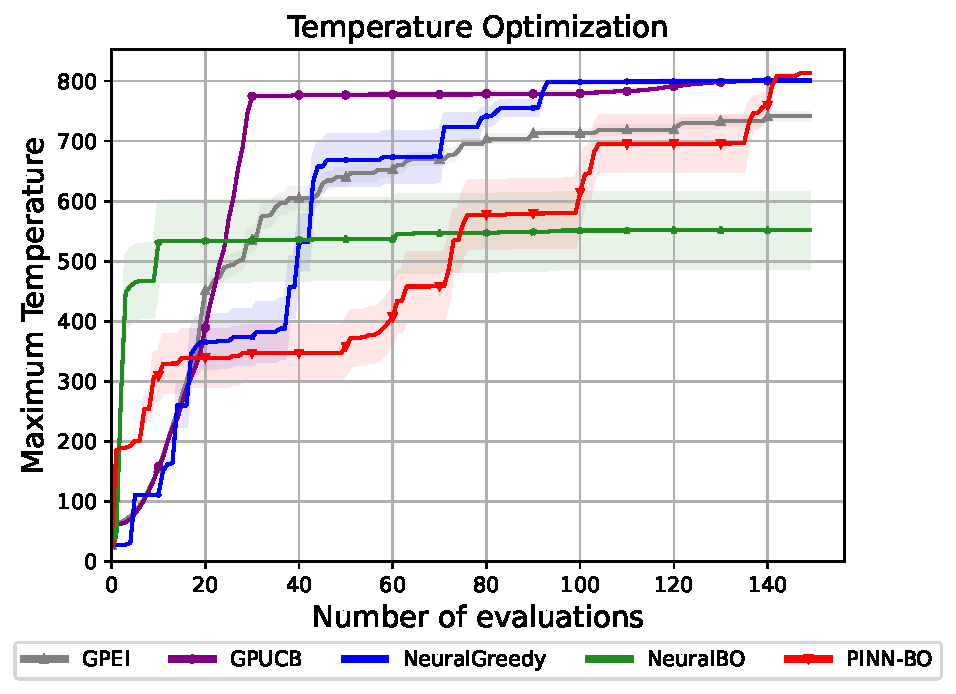
\includegraphics[width=\textwidth]{Figures/PINN-BO/Heat_dim_2_bc3.pdf}
        \caption{Temperature Optimization in case of boundary conditions 3}
        \label{fig:heat_3_opt}
    \end{subfigure}
    \caption{The figure shows the temperature optimization results of our PINN-BO and other baselines. For all three cases with different positions of maximum temperature, our PINN-BO performs better than all other baselines.}
    \label{fig:heat_opt}
\end{figure}


\subsubsection{Optimizing Beam Displacement}
We present the benchmark optimization outcomes obtained through our proposed method, PINN-BO, and the baseline approaches, addressing the task of minimizing the deflection of a non-uniform Euler-Bernoulli beam. The governing differential equation describing the behavior of a non-uniform Euler-Bernoulli beam is provided below: 
\begin{equation*}
    \frac{d^2}{dx^2} \left( EI(x) \frac{d^2 w(x)}{dx^2} \right) = q(x),
\end{equation*}
where
$EI(x)$ represents the flexural rigidity of the beam, which can vary with position $x$, and $w(x)$ represents the vertical displacement of the beam at position $x$ and 
$q(x)$ represents the distributed or concentrated load applied to the beam. 
In our implementation, we consider the detailed expression of $\text{EI}(x)$ and $q(x)$ as follows:
\begin{align*}
    \text{EI}(x) &= \frac{e^x}{\rho(x)},\\
    \rho(x) &= 2.4 x - 64 \pi^{2} e^{4 x} \sin{\left(4 \pi e^{2 x} \right)} - 396 e^{2 x} \sin{\left(20 x \right)} \\
    &+ 80 e^{2 x} \cos{\left(20 x \right)} + 16 \pi e^{2 x} \cos{\left(4 \pi e^{2 x} \right)} + 0.4
\end{align*}
We employed the Finite Difference Method (FDM) to solve the non-uniform Euler-Bernoulli beam equation. It's crucial to note that this step is solely for generating observations at each input point. Despite obtaining this solution, our methods and all baseline techniques continue to treat this solution as a black-box function, accessing observations solely through querying. In Figure \ref{fig:beam_illustration}, the displacement values $w(x)$ for $x \in (0,1)$ are illustrated. The optimization results for both our PINN-BO and the other baseline methods are presented in Figure \ref{fig:beam_opt}.
\clearpage
\begin{figure}[!t]
    \centering
    \begin{subfigure}[t]{0.44\textwidth}
        \centering
    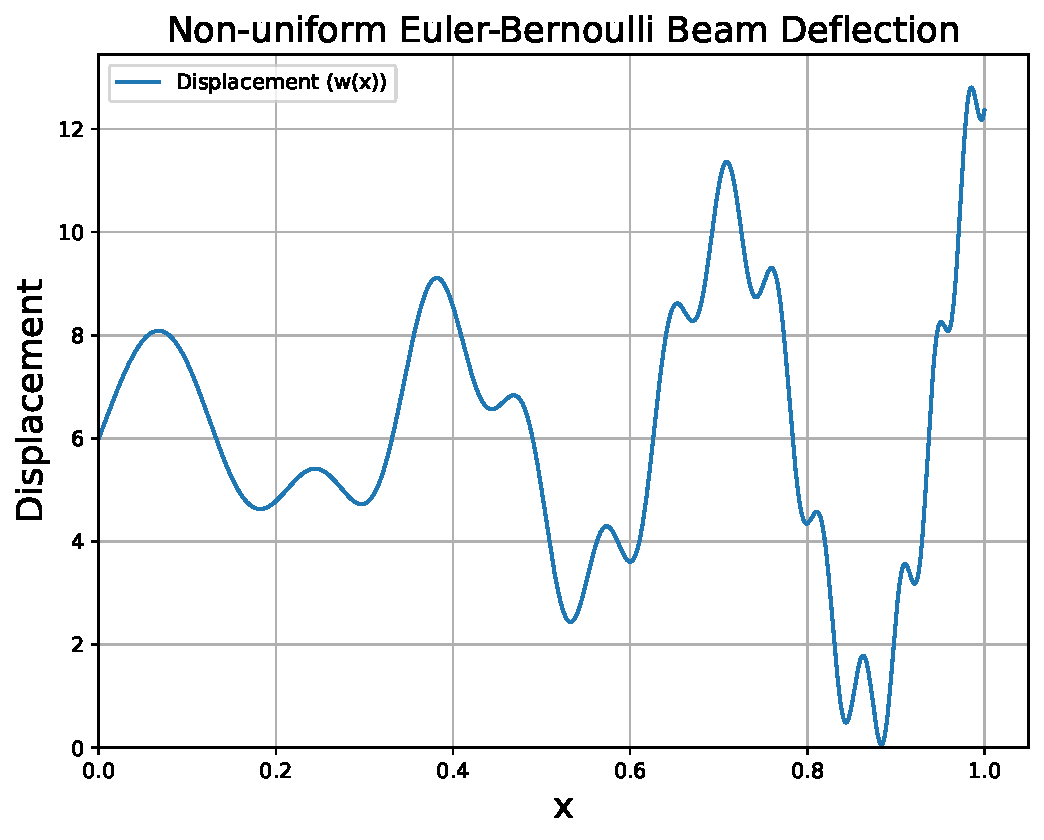
\includegraphics[width=\textwidth]{Figures/PINN-BO/beam.pdf}
    \caption{Displacement of non-uniform Euler beam}
     \label{fig:beam_illustration}
    \end{subfigure}
    \hfill
    \begin{subfigure}[t]{0.49\textwidth}
        \centering
        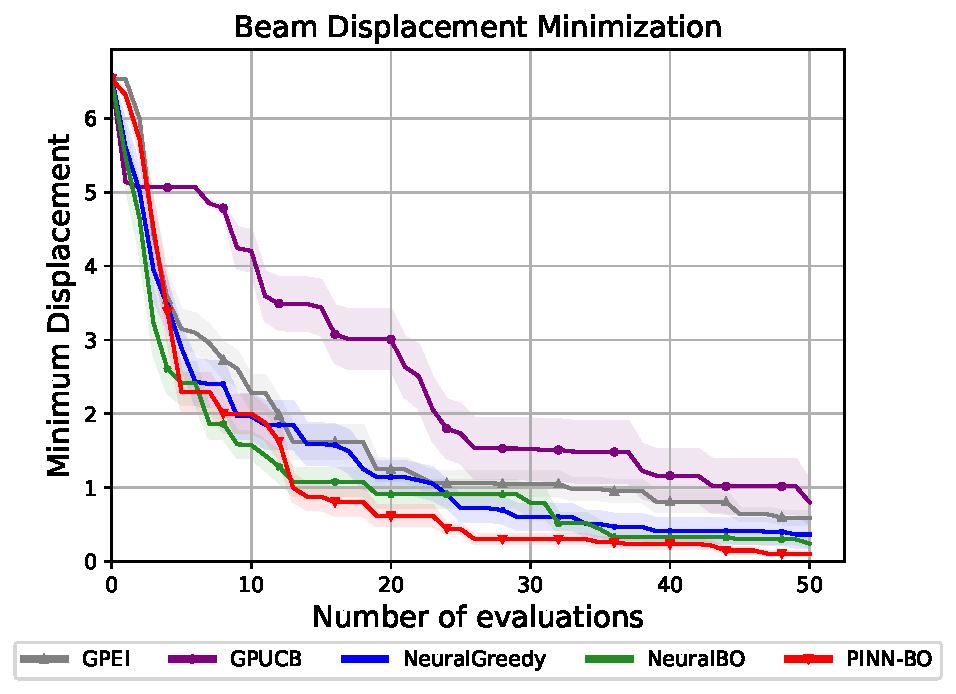
\includegraphics[width=1\textwidth]{Figures/PINN-BO/BeamDeflection_dim_1.pdf}
        \caption{Displacement Optimization of non-uniform Euler beam}
        \label{fig:beam_opt}
    \end{subfigure}
    \caption{Displacement of a non-uniform Euler Beam and minimum displacement found by our PINN-BO and the other baselines. The left panel illustrates the natural displacement profile of the non-uniform Euler beam under given loads $q(x)$,  flexural rigidity $EI(x)$, and boundary conditions. The right panel depicts the optimized position on the beam where the displacement is minimized, highlighting the location where the structural response is at its lowest.}
    \label{fig:beam}
\end{figure}



%  The steady-state heat equation is given by: $\nabla^2 T(x, y) = 0$, 
%  In this paper, our task is to find the best position $(x,y)$ that maximizes temperature $T$ within the defined domain. Formally, this problem can be defined as: 
% \begin{equation*}
%         \underset{x,y \in \mathcal{U}}{\max}  \;T(x,y) \text{ s.t. }  \nabla^2 T(x, y) = 0,
% \end{equation*}
% The details and the results of optimizing these heat equation problems are provided in Section A.2. The optimization results of our PINN-BO, in comparison to other baseline methods, for the first case of the heat equation, are depicted in Figure \ref{fig:heat_main}.

% \begin{figure}
%   \centering
%   \begin{subfigure}[t]{0.48\textwidth}
%     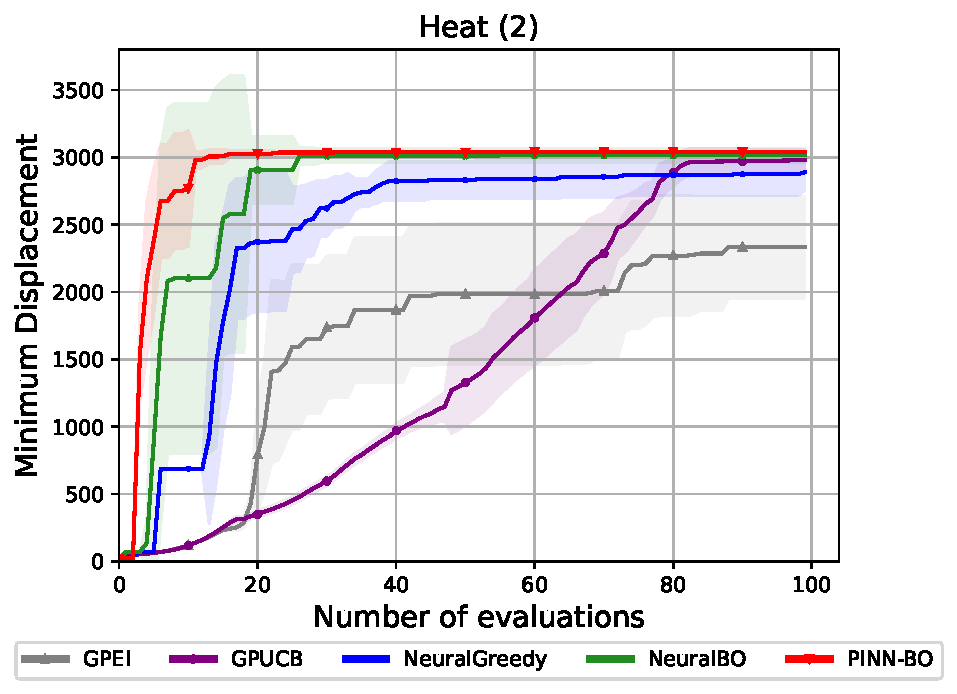
\includegraphics[width=\textwidth]{Figures/PINN-BO/Heat_dim_2.pdf}
%   \caption{The optimization results for finding the maximum temperature comparing the proposed PINN-BO with the baselines. It can be seen that, using the \ac{pde} heat equation, PINN-BO found the maximum temperature faster than all baselines.}
%   \label{fig:heat_main}
%   \end{subfigure}
%   \hfill
%   \begin{subfigure}[t]{0.48\textwidth}
%     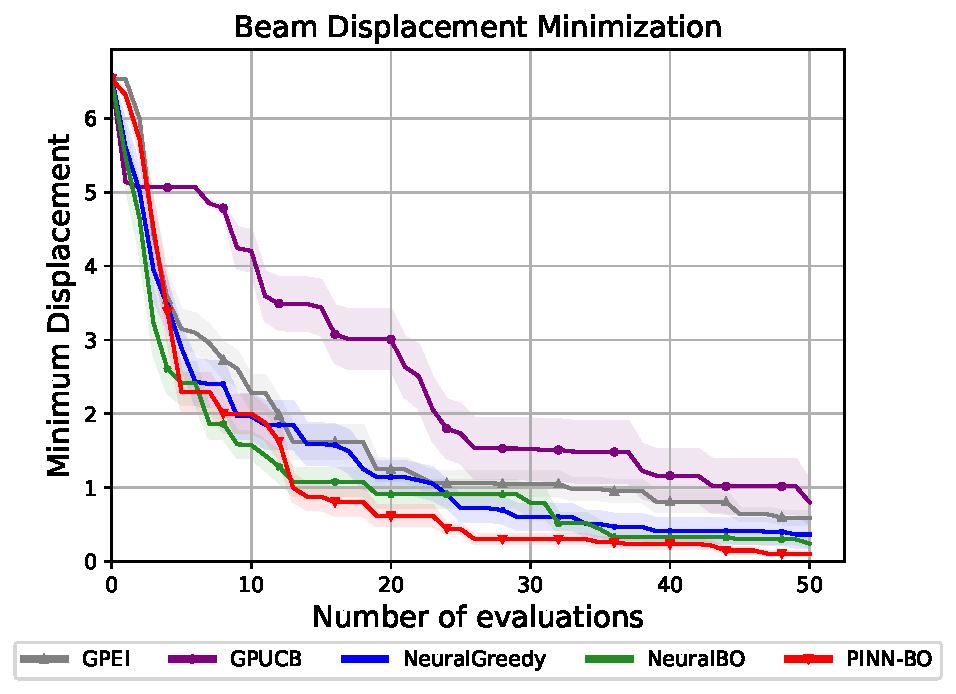
\includegraphics[width=\textwidth]{Figures/PINN-BO/BeamDeflection_dim_1.pdf}
%   \caption{The minimum displacement on the non-uniform Euler beam under given loads $q(x)$,  flexural rigidity $EI(x)$, and boundary conditions. In comparison with other baselines, our proposed PINN-BO found the location with the smallest displacement, ensuring stability when placing the load over the beam.}
%   \label{fig:beam_main}
%   \end{subfigure}
%   \caption{The optimization results for real-world applications comparing the proposed PINN-BO with the baselines.}
% \end{figure}

% \subsubsection{Optimizing Beam Displacement}
% Euler-Bernoulli beam theory is a widely used model in engineering and physics to describe the behavior of slender beams under various loads. The governing differential equation for a non-uniform Euler-Bernoulli beam is given by: 
% \begin{equation*}
%     \frac{d^2}{dx^2} \left( EI(x) \frac{d^2 w(x)}{dx^2} \right) = q(x),
% \end{equation*}
% where
% $EI(x)$ represents the flexural rigidity of the beam, which can vary with position $x$, and $w(x)$ represents the vertical displacement of the beam at position $x$, and $q(x)$ represents the distributed or concentrated load applied to the beam. The lower value deflection leads to a stiffer and more resilient structure, hence reducing the risk of structural failure and serviceability issues.  In this paper, we consider the task of finding the position $x$ that minimizes displacement $w(x)$. This problem can be defined as: 
% \begin{align*}
%     \underset{x \in \mathcal{S}}{\min}  \;
%         w(x) \\
% \text{ s.t. }  \frac{d^2}{dx^2} \left( EI(x) \frac{d^2 w(x)}{dx^2} \right) = q(x)
% \end{align*}


% \section{Conclusion}
% \label{section:pinn-bo_conclusion}
% We introduced a novel black-box optimization scenario incorporating \acfp{pde} as additional information. Our solution, PINN-BO, is a new algorithm tailored to this challenge. We conducted a theoretical analysis, demonstrating its convergence with a tighter regret bound. Through experiments involving synthetic benchmark functions and real-world optimization tasks, we validated the efficacy of our approach. Our method, due to using a neural network, is applicable to a broad set of optimization problems where the input space is complex (e.g. drug discovery), and can significantly accelerate the optimization by leveraging the auxiliary knowledge via \acp{pde}.  
